Skifter
- DONE - kør alberts kode for at sikre vi får de tal som vi mangler (MAE for ARIMA og AIC for GETS modellen)
- Done - omskriv gets afnsit så det passer med de nye data
- Done - sæt den fulde gum modellen i appendix, og referer til den
- Done - Tjek lige hvilken periode dummyen er på? Er det step dummy der er 1 fremover eller er den 1 i en periode under corona?

Svar:
Det er en vindues-dummy (WIN) — altså 1 kun i en afgrænset periode, 0 ellers.

Konkret fra 05_arima_forecasts:

full_xreg <- make_break_xreg(
  dates       = df_full$date,
  break_dates = as.Date("2021-04-01"),
  end_dates   = as.Date("2023-12-31"),
  type        = "WIN"
)
Så dummyen er:

1 fra april 2021 til december 2023 (corona/surge-perioden)
0 alle andre måneder — både før og efter
Det er altså ikke en step-dummy der bliver hængende på 1 fremover. Den slukker igen når surgen er ovre.


- Done - Lav et forecasting plot af GETS modellen og smid i Appendix
- Done - Sikre at model 4 (GETS modellen) betaerne er korrekte og at teksten rundt om passer + slet ligningen



Egon
- Tilføj Alberts pointe omkring at undlade corona periode i dyn reg modellerne, hvis vi havde mere tid



Seb
- lav residualplot på ARIMA modellerne + evt dynreg modellerne
- done -> Opdater ADF test og undersøge hvad der sker med levels og at tallene i testene ændre sig fra tabel 3.2 til 3.3
- Done ->tilføje en forklarende sætning i teksten om hvorfor tallene i ADF og KPSS ændrer sig på inflations tidsserierne




Alle:














% ============================================================
%  3. DATA
% ============================================================
\chapter{Data}\label{sec:data}
The analysis in this paper draws on two monthly time series sourced from Eurostat, covering Denmark and the EU27 over the period from December 2000 to March 2026. The former is the Harmonised Index of Consumer Prices (HICP), measured as the annual rate of change in percent \parencite{eurostat_hicp}. The latter is the monthly unemployment rate, expressed as a percentage of the labour force for both sexes and all ages, not seasonally adjusted \parencite{eurostat_unemployment}. The estimation sample is restricted to the common observation period beginning in December 2000 due to data availability constraints in the European inflation series. 
\begin{table}[h!]
\centering
\small{
\caption{Data sources. All series are retrieved directly from Eurostat.}
\begin{tabular*}{\textwidth}{@{\extracolsep{\fill}}lll}
\hline \hline
\rule{0pt}{12pt}\textbf{Series} & \textbf{Region} & \textbf{Definition} \\ [3pt]
\hline
\rule{0pt}{12pt}Unemployment rate & Denmark & Eurostat harmonised, Total, monthly \\ [3pt]
\rule{0pt}{12pt}Unemployment rate & EU (27 countries)  & Eurostat harmonised, Total, monthly \\ [3pt]
\rule{0pt}{12pt}HICP rates of change & Denmark  & Eurostat harmonised, not seas.\ adj., monthly \\ [3pt]
\rule{0pt}{12pt}HICP rates of change &  EU (27 countries)  & Eurostat harmonised, not seas.\ adj., monthly \\ [3pt]
\hline \hline
\end{tabular*}
}
\end{table}

\section{Inspections of Raw Data}
\paragraph{Looking for trend}
Figure~\ref{fig:raw_data} shows the four unaltered series from December 2000 to March 2026. Danish and EU27 HICP inflation track each other closely over the sample period, remaining within 0 to 4 percent before surging to c.\ 10 and 12 percent, respectively, in 2022 amid post-COVID supply disruptions and energy price shocks, and have since retreated toward pre-shock levels. Neither series displays a clear deterministic trend. Their apparent co-movement motivates the inclusion of EU27 HICP inflation as a predictor in the multivariate framework.

Danish and EU27 unemployment display markedly different dynamics. EU27 unemployment follows a clear downward trend, peaking at 11 to 12 percent during the European sovereign debt crisis in 2012 and 2013 before declining steadily thereafter. Danish unemployment, by contrast, exhibits a more cyclical pattern within a narrower band, with the 2008 to 2009 financial crisis visible as an upward shift followed by a gradual recovery. The divergent dynamics suggest that domestic and European labour market conditions carry distinct information for Danish inflation forecasting.
\begin{figure}[H]
    \centering
    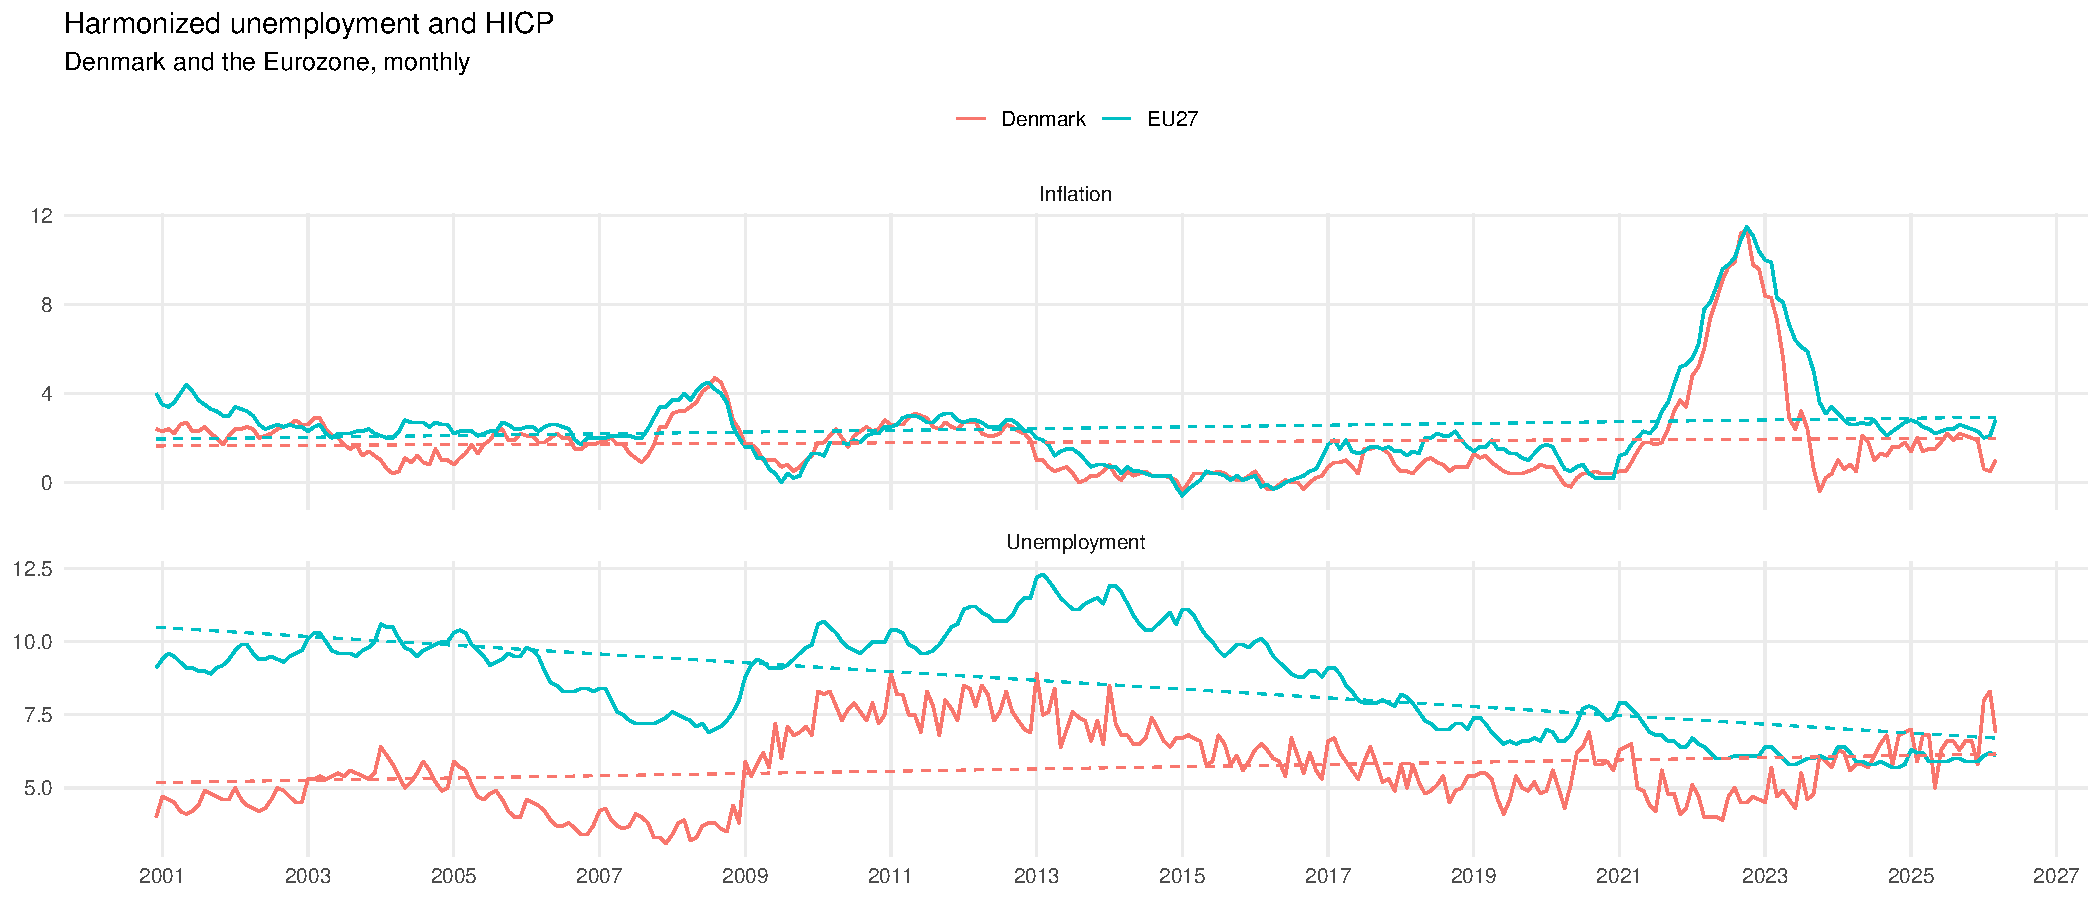
\includegraphics[width=1\linewidth]{billeder/facet_plot.pdf}
    \caption{Faceted plot of European and Danish inflation and unemployment.}
    \label{fig:raw_data}
\end{figure}
The time series plot in Figure~\ref{fig:raw_data} reveals the co-movement between Danish and EU27 inflation throughout the sample. 
Both series declined toward zero in the aftermath of the 2008 financial crisis, 
briefly turned negative around 2015, and surged sharply in 2022 before 
retreating. The EU27 series reached a slightly higher peak of approximately 
12 percent compared to around 11 percent for Denmark, but the timing and shape 
of the shock are virtually indistinguishable. This close co-movement reflects 
Denmark's fixed exchange rate peg to the euro under ERM II and suggests that 
EU27 inflation may carry predictive information for Danish inflation. This motivates 
its inclusion as an additional predictor in the multivariate forecasting models.

\paragraph{Initial look at the Phillips curve}

The scatter plot reveals a weak negative relationship between Danish unemployment and Danish inflation over the sample period, consistent with the theoretical prediction of the Phillips curve. The fitted line slopes downward, suggesting that lower unemployment is on average associated with higher inflation. However, the relationship is far from tight. We see that the dispersion around the fitted line is substantial, and several observations with low unemployment are associated with very low or even negative inflation, while high inflation observations appear across the full range of unemployment rates. The post-COVID inflation surge is visible as a cluster of high inflation observations at relatively low unemployment levels in the upper left of the plot.

\begin{figure}[H]
    \centering
    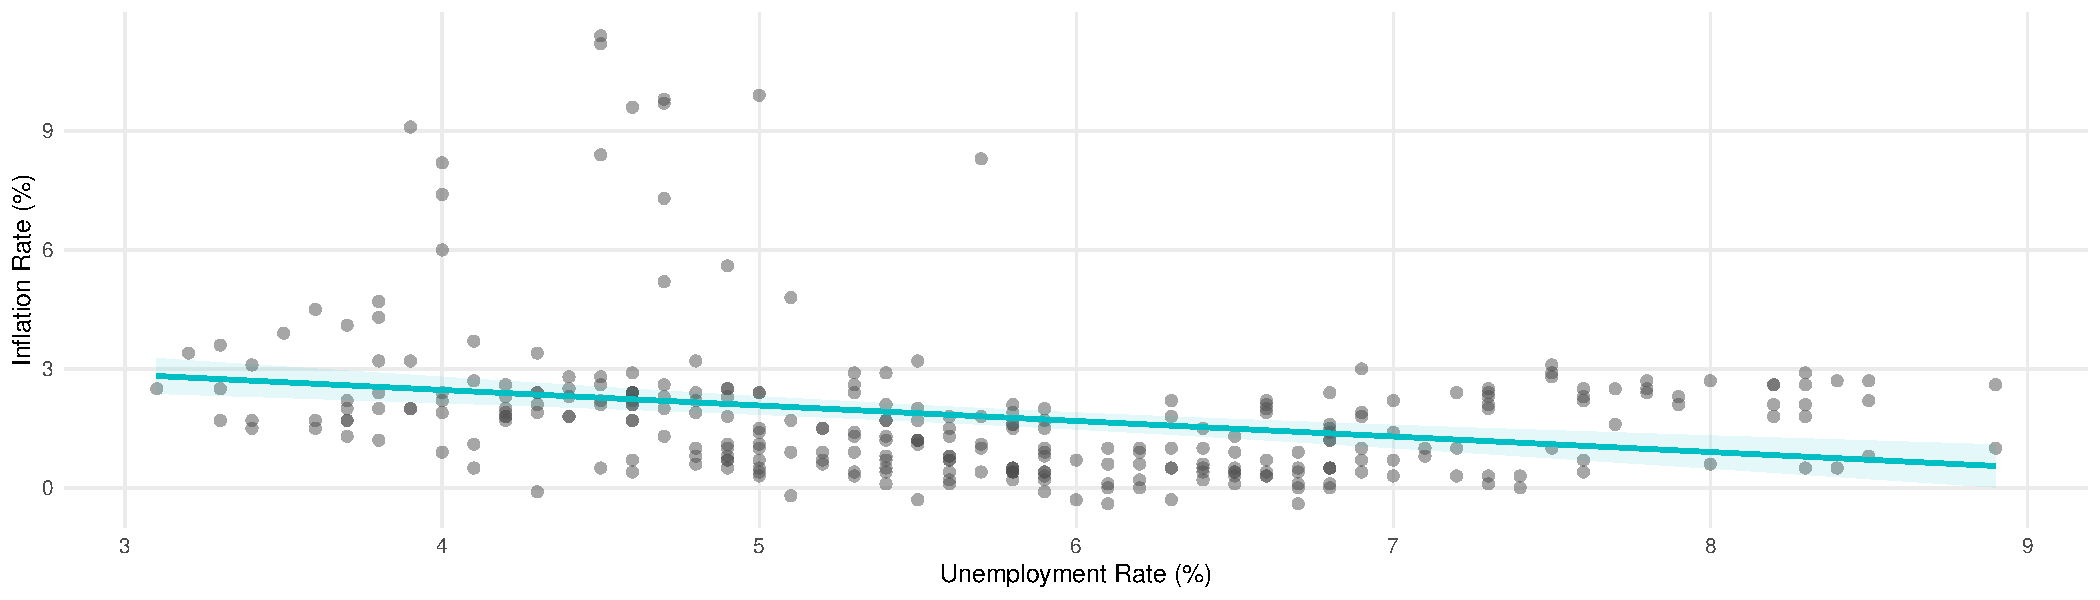
\includegraphics[width=\linewidth]{billeder/phillips.pdf}
    \caption{Scatter plot of Danish inflation against unemployment, with OLS fitted line.}
    \label{fig:02_philips_curve_denmark}
\end{figure}

The scatter plot suggests that while a negative correlation exists between the two series, unemployment alone explains little of the variation in Danish inflation. This motivates the use of a formal forecasting framework to assess whether unemployment retains predictive value for inflation.

% \subsubsection{Danish and EU inflation co-movement}

% \ref{fig:03_denmark_vs_EU_inflation} plots Danish and EU27 inflation over the full sample. The two series track each other closely throughout, displaying near-identical cyclical patterns across all major inflation episodes. Both series declined toward zero in the aftermath of the 2008 financial crisis, briefly turned negative around 2015 amid falling energy prices and deflationary pressure in the euro area, and then surged sharply in 2022 before retreating. The EU27 series reached a slightly higher peak of approximately 12 percent compared to around 11 percent for Denmark, but the timing and shape of the shock are virtually indistinguishable.

% % \begin{figure}[h]
% %     \centering
% %     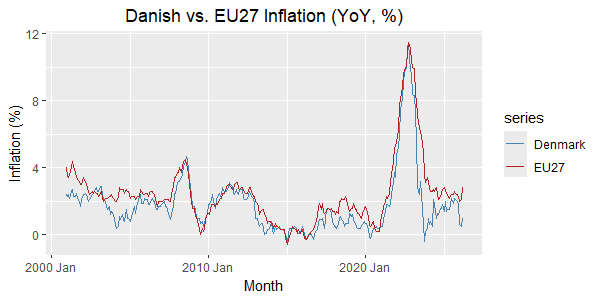
\includegraphics[width=0.5\linewidth]{billeder/03_denmark_vs_EU_inflation.png}
% %     \caption{Danish and European inflation}
% %     \label{fig:03_denmark_vs_EU_inflation}
% % \end{figure}

% The close co-movement reflects Denmark's deep integration with the European economy and its fixed exchange rate peg to the euro under ERM II, which ties Danish monetary conditions closely to those of the euro area. This suggests that EU27 inflation may carry predictive information for Danish inflation, motivating its inclusion as an additional predictor in the 
% multivariate forecasting model.

\paragraph{Looking for seasonality}


% ==== Bare lidt forklaring af dem hver  ======
% For Danish unemployment, there appears to be a mild seasonal pattern. Unemployment is often higher in the winter and early spring months, then tends to fall toward the summer, especially around June–August. However, the lines are quite noisy, so the seasonal pattern is not perfectly consistent across years.

% For Euro-area unemployment, the seasonal pattern is clearer. Many yearly lines decline from January/February toward the summer months and then rise again toward the end of the year. This suggests unemployment is typically lower in summer and higher in winter.

% For Danish inflation, there is no strong common seasonal pattern across years. Most yearly lines are clustered around relatively low inflation rates, while the years around COVID-19 show much higher inflation and dominate the plot. These outlier years reflect the unusual macroeconomic period rather than regular seasonality.

% For Euro-area inflation, the same applies. There is some variation across months, but the pattern is not stable across years. A few high-inflation years create visible spikes, especially later in the year, but this should not be interpreted as normal seasonal behavior

The seasonal plots indicate some recurring seasonal variation in unemployment, particularly for the euro area, where unemployment tends to be higher in winter and lower during the summer months. The pattern is weaker for Danish unemployment. In contrast, inflation displays less systematic seasonality. The inflation plots are dominated by a few high-inflation years, suggesting that variation is driven more by macroeconomic shocks than by stable monthly seasonal patterns.

\begin{figure}[H]
    \centering
    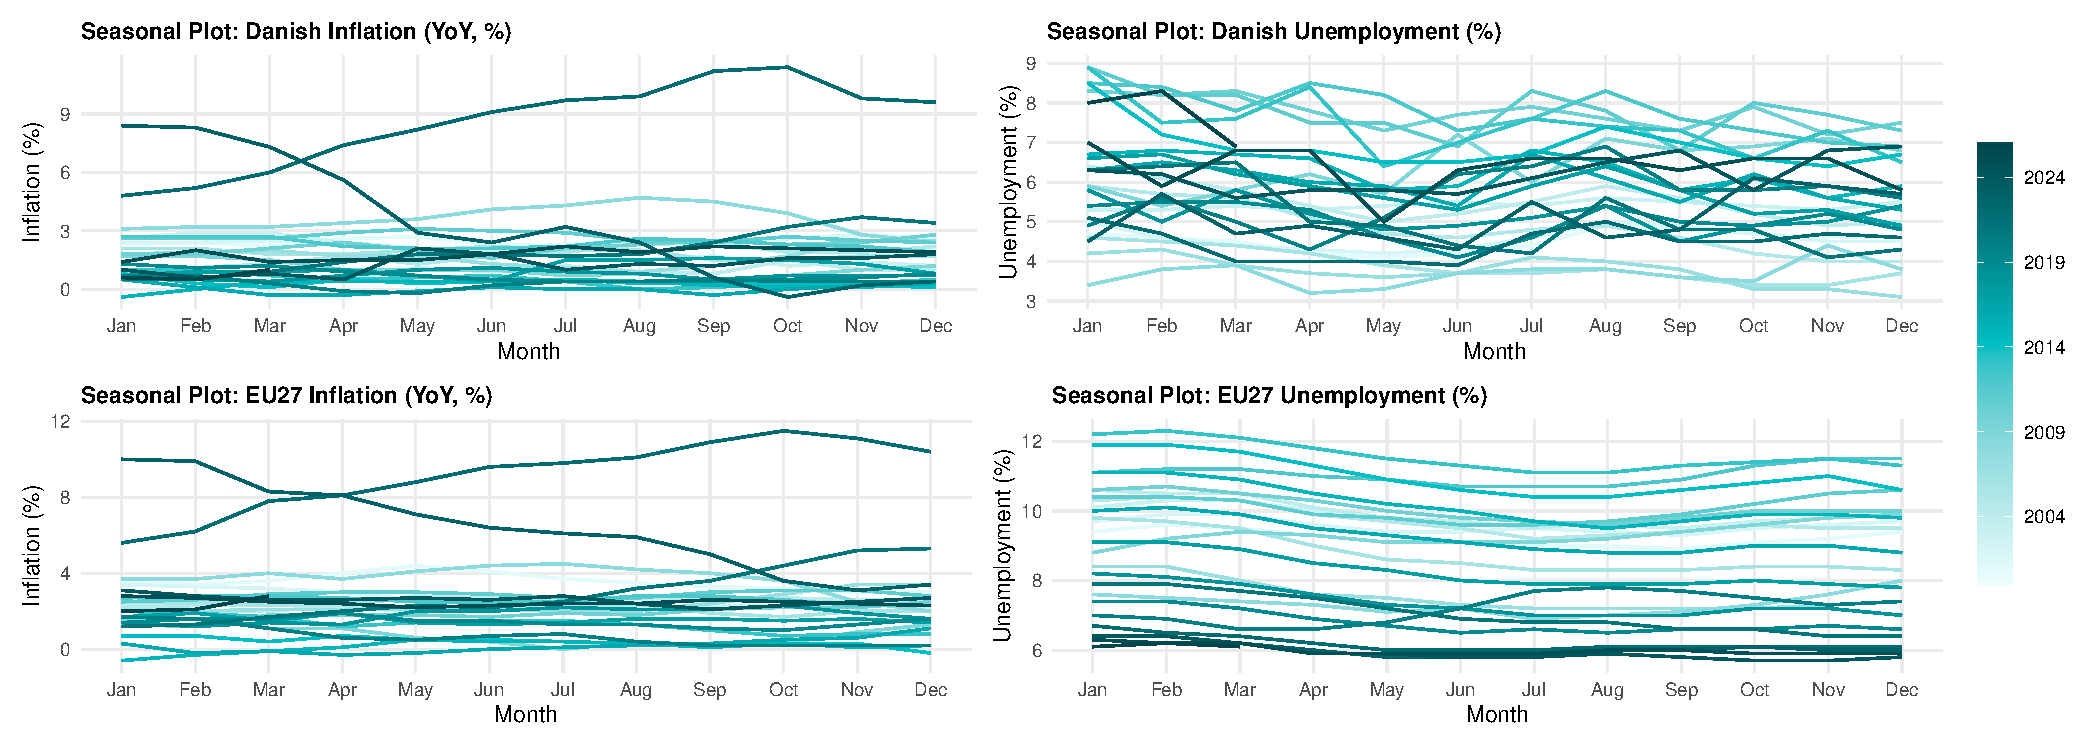
\includegraphics[width=1\linewidth]{billeder/subseason.pdf}
    \caption{Unemployment shows some seasonal behavior, especially in the euro area, while HICP shows little clear seasonality in this plot.}
    \label{fig:index_seasonal_plot}
\end{figure}
%\textcolor{red}{tænker jeg bare lige smider nogle subsires plots i appendix}
% ==== subseries seasonal plot 

% jeg ved ikke om der er plads til dette - ellers skal vi droppe de seasonal plots som 

% To examine this pattern more clearly, we next consider seasonal subseries plots, which compare observations within each calendar month over time. These plots confirm that unemployment contains a modest seasonal component, while inflation displays little evidence of stable seasonality. The inflation series are instead dominated by specific high-inflation episodes rather than regular monthly movements.



% \textcolor{red}{grafer skal fikses - tilføj at alle seasonal subseries plots can be seen in the appendix in \ref{fig: All seasonal subseries plots}}

% \begin{figure}[H]
%     \centering
%     \includegraphics[width=1\linewidth]{billeder/Danishunemploymentseasonalsubseries.png}
%     \caption{The plots confirm that unemployment contains a modest seasonal component, while inflation displays little evidence of stable seasonality}
%     \label{fig:seasonal_subseries_plot}
% \end{figure}
\paragraph{Testing for stationarity}

Before estimating the forecasting models, we assess stationarity using both the Augmented Dickey-Fuller (ADF) test and the KPSS test. The ADF test has non-stationarity as the null hypothesis, while the KPSS test has stationarity as the null hypothesis.



\begin{table}[H]
\centering
\small{
\caption{Stationarity tests}
\begin{tabular*}{\textwidth}{@{\extracolsep{\fill}}lcccc}
\hline \hline
\rule{0pt}{12pt}\textbf{Variable} & \textbf{ADF p-value} & \textbf{ADF conclusion} & \textbf{KPSS p-value} & \textbf{KPSS conclusion} \\ [3pt]
\hline
\rule{0pt}{12pt}Danish inflation, level      & $<0.01$ & Stationary     & $>0.10$ & Stationary     \\ [3pt]
\rule{0pt}{12pt}EU27 inflation, level        & $0.022$ & Stationary     & $>0.010$ & Non-stationary \\[3pt]
\rule{0pt}{12pt}Danish unemployment   & $0.821$ & Non-stationary & $0.012$ & Non-stationary \\[3pt]
\rule{0pt}{12pt}EU27 unemployment     & $0.827$ & Non-stationary & $<0.01$ & Non-stationary \\[3pt]
\hline \hline
\label{tab:stationarity_levels}
\end{tabular*}
}
\end{table}
The stationarity tests broadly confirm what the time series plots suggest. Both unemployment series are non-stationary without transformation, according to both the ADF and KPSS tests, and will be first-differenced prior to estimation. The inflation series, sourced directly as year-on-year rates of change, are already stationary transformations of the underlying price indices. Danish inflation is confirmed stationary by both tests, while EU27 inflation yields mixed results, though this is not uncommon given the sharp but transitory nature of the 2022 inflation surge. Both inflation series are used in levels throughout the analysis.






\paragraph{Reaching stationarity} Before estimating the forecasting models, we assess the stationarity properties of the series using both formal tests and graphical inspection of the ACF and PACF. The ADF test is used to test the null hypothesis of a unit root, while the KPSS test is used to test the null hypothesis of stationarity. The ACF and PACF plots are included as a graphical supplement, since slowly decaying autocorrelations may indicate non-stationarity or remaining seasonal dependence. The corresponding ACF and PACF plots are shown in Appendix~\ref{sec:appendix_acf_pacf}.


The inflation series are measured as year-on-year rates of change and are used in levels throughout the analysis. The unemployment series are non-stationary in levels and are therefore transformed using first differences:
\[
\Delta y_t = y_t - y_{t-1}.
\]
Seasonal differencing was also considered due to indications of annual dependence in the seasonal plots and ACFs. However, first differencing provided clearer evidence of stationarity for the unemployment series. Any remaining seasonal dynamics are therefore handled in the modelling stage, for example through seasonal ARIMA errors, rather than by applying seasonal differencing mechanically.

\begin{table}[H]
\centering
\small{
\caption{Stationarity tests for variables used in the models}
\begin{tabular*}{\textwidth}{@{\extracolsep{\fill}}lcccc}
\hline \hline
\rule{0pt}{12pt}\textbf{Variable} & \textbf{ADF p-value} & \textbf{ADF conclusion} & \textbf{KPSS p-value} & \textbf{KPSS conclusion} \\ [3pt]
\hline
\rule{0pt}{12pt} Danish inflation, level          & $<0.01$ & Stationary & $>0.10$ & Stationary \\ [3pt]
\rule{0pt}{12pt}EU27 inflation, level            & $0.022$ & Stationary & $>0.10$ & Stationary \\ [3pt]
\rule{0pt}{12pt}Danish unemployment, first diff. & $<0.01$ & Stationary & $>0.10$ & Stationary \\ [3pt]
\rule{0pt}{12pt}EU27 unemployment, first diff.   & $<0.01$ & Stationary & $>0.10$ & Stationary \\ [3pt]
\hline \hline
\end{tabular*}}
\label{tab:stationarity_tests}
\end{table}

The results indicate that the inflation series can be treated as stationary in levels, whereas the unemployment series require first differencing. This transformation ensures that the external regressors used in the dynamic regression models are stationary. The marginal shift in the EU27 inflation results between Table~\ref{tab:stationarity_levels} and Table~\ref{tab:stationarity_tests} reflects that the test statistics for this borderline series are sensitive to the lag specification and the post-surge observations included in each test; the series sits close to the critical region in both cases, but the evidence taken together supports treating it as stationary in levels for the purposes of the dynamic regression models. The ACF and PACF plots, reported in the appendix, support this conclusion and also indicate that some seasonal dependence remains, which is addressed in the model specification rather than through additional seasonal differencing.
